%% 
%% Copyright 2019-2020 Elsevier Ltd
%% 
%% This file is part of the 'CAS Bundle'.
%% --------------------------------------
%% 
%% Supplementary material for cas-sc documentclass
%% 

\documentclass[a4paper,fleqn]{cas-sc}
\pdfminorversion=7

\usepackage{tablefootnote}
\usepackage{appendix}
\usepackage{threeparttable}
\usepackage{afterpage}
\usepackage[table]{xcolor}
\usepackage{float}
\usepackage[authoryear]{natbib}
\usepackage{caption}
\captionsetup{format=plain, indention=0pt}
\hypersetup{
	colorlinks=true,
	linkcolor=blue,
	filecolor=magenta,      
	urlcolor=cyan,
	citecolor=blue,
}
\usepackage{tabularx}
\usepackage{longtable}
\usepackage{tabulary}
\usepackage{placeins}
\usepackage{microtype}
\setlength{\emergencystretch}{2em}
\usepackage[nameinlink]{cleveref}
\Crefname{figure}{Fig.}{Figs.}
\crefname{figure}{fig.}{figs.}
\Crefname{equation}{Eq.}{Eqs.}

\renewcommand{\thesection}{S\arabic{section}}
\renewcommand{\thetable}{S\arabic{table}}
\renewcommand{\thefigure}{S\arabic{figure}}
\renewcommand{\theequation}{S\arabic{equation}}

%%%Author macros
\def\tsc#1{\csdef{#1}{\textsc{\lowercase{#1}}\xspace}}
\tsc{WGM}
\tsc{QE}
\tsc{EP}
\tsc{PMS}
\tsc{BEC}
\tsc{DE}
%%%

\usepackage{xr}
\externaldocument[main-]{cas-sc-template}

\begin{document}
\ExplSyntaxOn
\bool_gset_true:N \g_stm_nologo_bool
\ExplSyntaxOff
\let\printorcid\relax
\let\WriteBookmarks\relax
\def\floatpagepagefraction{1}
\def\textpagefraction{.05}
\setcounter{topnumber}{4}
\setcounter{bottomnumber}{3}
\setcounter{totalnumber}{8}
\renewcommand{\topfraction}{0.92}
\renewcommand{\bottomfraction}{0.85}
\renewcommand{\textfraction}{0.08}
\renewcommand{\floatpagefraction}{0.75}

\shorttitle{Supplementary material}
\shortauthors{A. Xu et al.}

\title [mode = title]{Supplementary Material: Beyond Static Imitation: Auditing LLM-Derived Traveler Responses for Transport Simulation}

\author[1]{An Xu}
\ead{AnX.RTL2324@tum-asia.edu.sg}

\author[2]{Zekai Jin}

\author[2]{Chengbo Zhang}

\author[1]{Yunfei Yin}
\cormark[1]
\ead{yunfeiyin@hit.edu.cn}

\address[1]{School of Transportation Science and Engineering, Harbin Institute of Technology, Harbin 150090, China}
\address[2]{Department of Civil Engineering, McGill University, Montreal, QC H3A 0C3, Canada}

\cortext[cor1]{Corresponding author: Yunfei Yin (yunfeiyin@hit.edu.cn).}

\begin{abstract}
This supplement documents the traveler inputs and stated-choice tasks, the specification and training of the Student models, the complete comparisons with stated choices and with the contemporary Teacher, the simulation experiments and the computational measurements. It follows the order of the three questions in the main article, which concern fidelity to Teacher responses, agreement with stated responses and preservation of responses in simulation.
\end{abstract}
\maketitle
\section{Encoded field dictionary}
\label{sec:field_dictionary}
The questionnaire tasks, sample flow, route-search definitions and input sensitivity are in Appendix~\ref{main-sec:supp_inputs} of the article. This section retains the field-level dictionary for reproduction.
\begin{table}[pos=htbp]
\centering\small
\caption{Fields of the encoded traveler state. Mode availability is represented separately from these attributes.}
\label{tab:input_dictionary}
\renewcommand{\arraystretch}{1.12}
\begin{tabularx}{\linewidth}{@{}p{0.25\linewidth}X@{}}
\toprule
Input group & Fields \\
\midrule
Categorical traveler fields & age group, income group, occupation, habitual mode, schedule flexibility, mobility limitation \\
Categorical trip/context fields & trip purpose, time constraint, weather condition \\
Numerical traveler fields & household size, presence of children, car ownership, driving licence, bicycle ownership, transit pass \\
Numerical trip fields & distance (km), desired departure time, desired arrival time \\
Numerical context fields & weather intensity, road congestion, PT delay, PT disruption, road disruption, fare multiplier, parking cost multiplier, congestion charge \\
Alternative fields & travel time, monetary cost, access time, number of transfers, reliability delay, weather exposure \\
Additional PT-supply fields & PT feasibility, egress time, waiting time, in-vehicle time, transfer time, coverage ratio \\
\bottomrule
\end{tabularx}
\par\smallskip\begin{minipage}{\linewidth}\footnotesize
The nine categorical and seventeen global numerical fields form the shared state; each mode has twelve numerical attributes. Times are in minutes and distance in kilometres before encoding. Categorical vocabularies and numerical normalization are fitted on training data. For SA-Student, existing statistics are inherited and only the six added supply fields receive newly fitted normalization. The supplementary data files give the variable names used in the implementation.
\end{minipage}
\end{table}

\FloatBarrier

\section{Controlled learning and departure prediction}
\label{sec:supp_controlled}
\subsection{Training and model selection}
The controlled benchmark contains 1,839 training, 365 validation and 437 test states from disjoint groups of 28, six and six personas. The test set comprises 226 single-context, 51 accessibility, 96 joint-context and 64 mechanism states, which define 398 response pairs and 94 interaction contrasts. Training proceeds over pairs, and the 1,681 training pairs expose the model to 3,362 states per epoch. Within each training seed (42, 2026 and 7), the four neural objectives share initialization, feature encoding, the order of training pairs and a budget of 6,360 updates over 120 epochs. They also share the availability rule, under which a mode enters the response loss if it is available in either state of a pair.

Every neural Student has 24,562 parameters. The nine categorical fields receive eight-dimensional embeddings and are combined with 17 standardized global features in a two-layer encoder of width 64. A mode embedding and the 12 alternative attributes enter a two-layer encoder of width 32, and a scorer with 64 hidden units maps both representations to utilities. The departure predictor uses the global representation together with the mean representation of the available alternatives. Hidden layers use ReLU activations, and the global encoder and scorer apply a dropout rate of 0.1. All models are trained with Adam at a learning rate of $1.25\times10^{-4}$ and weight decay of $10^{-4}$, in batches of 32 pairs, with a Huber loss on departure adjustment whose transition is one minute. For the probability-response comparison, the epoch with the lowest validation macro-source KL is retained.

MNL-S specifies four linear utilities over 111 explanatory variables. It minimizes cross-entropy against the soft Teacher targets with an $L_2$ penalty, whose weight of $10^{-4}$ was chosen from $\{10^{-4},10^{-3},10^{-2},10^{-1}\}$ by validation macro-source KL. Estimation by L-BFGS-B converges within 2,000 iterations. The ridge departure predictor uses a penalty of $10^{-3}$, chosen by validation departure MAE. Table~\ref{tab:matched_diagnostics} reports feasibility and departure-tail metrics for the models selected on choice.
\begin{table}[pos=htbp]
\centering\small
\caption{Construction of the four behavioral-supervision sources and their contributions to the controlled test set.}
\label{tab:training_sources}
\setlength{\tabcolsep}{4pt}
\renewcommand{\arraystretch}{1.16}
\begin{tabularx}{\linewidth}{@{}p{0.16\linewidth}Xrr@{}}
\toprule
Source & Comparison represented & States & Pairs \\
\midrule
Single-context & A traveler--trip baseline and single-axis changes in weather, congestion, PT delay, fares, parking or road disruption. & 226 & 214 \\
Accessibility & The same traveler and trip under PT supply profiles, varying access, waiting, transfers and connection feasibility. & 51 & 40 \\
Joint context & Two perturbations applied together, linked to their baseline and single-perturbation counterparts where available. & 96 & 96 \\
Mechanism & A baseline and three context--attribute variants: both changed, context only, or attributes only. These separate different encoded paths of the same intervention. & 64 & 48 \\
\midrule
Total & Held-out persona groups across the four sources. & 437 & 398 \\
\bottomrule
\end{tabularx}
\par\smallskip\begin{minipage}{\linewidth}\footnotesize
A state combines a traveler, a trip, a context, mode attributes and Teacher targets. A response pair links two states, and a state can belong to several pairs. Persona groups are disjoint across training, validation and test (28/6/6). Accessibility data additionally use disjoint OD pools. Teacher probability vectors are averaged over valid repeated queries. The counts are states and pairs, not independent travelers.
\end{minipage}
\end{table}


\paragraph{Response and feasibility metrics.}
\label{sec:metric_definitions}
For response pair $i$, let $\mathcal A_i$ be the set of alternatives available in either of its two states. Probability-response error is
\begin{equation}
 E_{\Delta p}=\frac{1}{N_{\mathrm{pair}}}\sum_{i=1}^{N_{\mathrm{pair}}}
 \frac{1}{|\mathcal A_i|}\sum_{m\in\mathcal A_i}
 |\Delta p^S_{im}-\Delta p^T_{im}|.
 \label{eq:response_metric}
\end{equation}
Fidelity at individual states is measured by $D_{\mathrm{KL}}(\mathbf p_T\Vert\mathbf p_S)=\sum_{m:p_{T,m}>0}p_{T,m}\log(p_{T,m}/p_{S,m})$, and macro-source KL summarizes this divergence at the level of the four supervision sources. For a linked baseline $0$, individual perturbations $a,b$ and their combination $ab$, the mode-specific interaction is
\begin{equation}
 I^j_{im}=p^j_{im}(ab)-p^j_{im}(a)-p^j_{im}(b)+p^j_{im}(0),\qquad j\in\{T,S\}.
 \label{eq:interaction_metric}
\end{equation}
Interaction error averages $|I^S_{im}-I^T_{im}|$ over the modes available in a linked contrast and then over the 94 evaluated contrasts. It therefore measures how two perturbations combine, rather than the response to a single intervention. With $\mathcal E$ denoting the test states in which no PT route is found, the feasibility violation rate is
\begin{equation}
 \mathrm{FVR}=\frac{1}{|\mathcal E|}\sum_{x\in\mathcal E}
 \mathbf 1\!\left\{\operatorname*{arg\,max}_{m\in\mathcal A(x)}p_{S,m}(x)=\mathrm{PT}\right\}.
 \label{eq:fvr_metric}
\end{equation}
The controlled evaluation contains $|\mathcal E|=12$ such states. FVR counts how often PT is the most probable mode where the route search finds no connection, which differs from the mean PT probability on those states. Departure MAE averages $|\tau_S-\tau_T|$ over the evaluated states.

\begin{table}[pos=htbp]
\centering\small
\caption{Feasibility and departure diagnostics on the same controlled test pool. Neural entries average three training seeds. FVR uses 12 infeasible states per seed. Departure errors are in minutes; response SD describes training-seed variation.}
\label{tab:matched_diagnostics}
\begin{tabular}{@{}lrrrr@{}}
\toprule
Model & FVR & Departure median & Departure P90 & Response SD \\
\midrule
Soft KL & 0.0833 & 5.12 & 15.59 & 0.0032 \\
CE + KL & 0.0833 & 5.16 & 15.74 & 0.0016 \\
Signed response & 0.0278 & 5.18 & 15.37 & 0.0050 \\
Direction + magnitude & 0.0556 & 5.06 & 16.06 & 0.0042 \\
MNL-S & 0.0000 & 10.53 & 25.42 & -- \\
\bottomrule
\end{tabular}
\end{table}


\subsection{Independent departure predictors}
\label{sec:departure_predictors}
The modular comparison keeps the 444 MNL-S choice coefficients fixed and adds either a bounded linear predictor with 111 parameters or an independent neural predictor with 18,289 parameters. The neural predictor keeps the feature encoders and departure layer of the joint architecture, omits the utility scorer and is trained on the departure Huber loss alone. The two modular Students therefore have 555 and 18,733 parameters in total.

All timing comparisons share the training states, the three seeds, the optimizer and the budget of 6,360 updates. The retained epoch minimizes validation departure MAE, with ties resolved in favour of the earliest epoch, and the four joint objectives are retrained under the same criterion. These timing fits are separate from the fits used for the probability-response comparison, although both follow the same update budget. Table~\ref{tab:departure_runs} lists the selected epochs, the results for every seed and the inference times, and Table~\ref{tab:departure_sources} breaks the errors down by supervision source.
\begin{table}[pos=htbp]
\centering\footnotesize
\caption{Timing models selected by validation departure MAE, evaluated on the 437 test states.}
\label{tab:departure_runs}
\setlength{\tabcolsep}{3pt}
\renewcommand{\arraystretch}{1.12}
\begin{tabular*}{\linewidth}{@{\extracolsep{\fill}}lrrrrrrrr@{}}
\toprule
Model & Seed & Epoch & MAE & Median & P90 & Parameters & Train (s) & Infer. ($\mu$s) \\
\midrule
Soft KL & 42 & 2 & 8.461 & 3.355 & 25.611 & 24562 & 29.9 & 2.00 \\
Soft KL & 2026 & 117 & 7.048 & 5.236 & 15.801 & 24562 & 27.3 & 2.39 \\
Soft KL & 7 & 31 & 7.315 & 5.395 & 16.061 & 24562 & 38.1 & 2.07 \\
CE + KL & 42 & 2 & 8.455 & 3.348 & 25.600 & 24562 & 33.1 & 1.40 \\
CE + KL & 2026 & 108 & 6.719 & 5.452 & 14.114 & 24562 & 38.5 & 2.23 \\
CE + KL & 7 & 36 & 7.103 & 5.110 & 15.388 & 24562 & 34.9 & 1.83 \\
Signed & 42 & 2 & 8.464 & 3.355 & 25.612 & 24562 & 33.8 & 1.91 \\
Signed & 2026 & 35 & 7.441 & 5.399 & 15.143 & 24562 & 33.2 & 1.78 \\
Signed & 7 & 30 & 7.239 & 5.255 & 15.938 & 24562 & 30.9 & 1.75 \\
Dir. + mag. & 42 & 2 & 8.459 & 3.339 & 25.592 & 24562 & 30.2 & 1.67 \\
Dir. + mag. & 2026 & 108 & 6.952 & 4.858 & 14.918 & 24562 & 34.6 & 1.79 \\
Dir. + mag. & 7 & 30 & 7.238 & 5.397 & 16.072 & 24562 & 30.2 & 1.89 \\
MNL + bounded & 42 & 56 & 10.237 & 8.226 & 19.171 & 555 & 2.4 & 0.20 \\
MNL + bounded & 2026 & 31 & 10.737 & 7.321 & 24.947 & 555 & 2.4 & 0.19 \\
MNL + bounded & 7 & 22 & 12.592 & 10.687 & 23.368 & 555 & 2.6 & 0.19 \\
MNL + neural & 42 & 2 & 8.423 & 3.282 & 25.563 & 18733 & 19.7 & 1.30 \\
MNL + neural & 2026 & 116 & 7.348 & 5.248 & 15.745 & 18733 & 19.8 & 1.91 \\
MNL + neural & 7 & 97 & 7.046 & 5.231 & 15.023 & 18733 & 23.7 & 1.82 \\
\bottomrule
\end{tabular*}
\par\smallskip{\footnotesize All timing errors are in minutes. Every run completes 120 epochs and 6,360 updates; Epoch identifies the minimum validation departure-MAE checkpoint. For the modular Students, parameters include the 444 fixed MNL choice coefficients and the timing predictor. Inference time is the median of 30 batches of the 437 encoded states divided by 437, after five untimed calls and with two CPU threads, excluding encoding and transport preparation. Concurrent workload limits cross-run timing comparisons.}
\end{table}


\begin{table}[pos=htbp]
\centering\footnotesize
\caption{Departure errors by test source under validation departure-MAE selection.}
\label{tab:departure_sources}
\setlength{\tabcolsep}{3pt}
\renewcommand{\arraystretch}{1.12}
\begin{tabular}{@{}llrrrr@{}}
\toprule
Model & Source & States & MAE & Median & P90 \\
\midrule
Soft KL & single-context & 226 & $6.849\pm0.667$ & 4.226 & 18.489 \\
Soft KL & joint & 96 & $8.923\pm2.010$ & 5.378 & 21.530 \\
Soft KL & mechanism & 64 & $5.921\pm0.466$ & 4.643 & 12.608 \\
Soft KL & accessibility & 51 & $10.614\pm0.732$ & 5.379 & 27.664 \\
CE + KL & single-context & 226 & $6.618\pm0.888$ & 4.282 & 17.240 \\
CE + KL & joint & 96 & $8.729\pm2.170$ & 5.319 & 21.548 \\
CE + KL & mechanism & 64 & $5.911\pm0.558$ & 4.546 & 12.851 \\
CE + KL & accessibility & 51 & $10.453\pm0.769$ & 5.354 & 27.870 \\
Signed & single-context & 226 & $6.964\pm0.553$ & 4.300 & 18.324 \\
Signed & joint & 96 & $9.186\pm1.845$ & 5.317 & 21.257 \\
Signed & mechanism & 64 & $5.843\pm0.352$ & 4.636 & 12.183 \\
Signed & accessibility & 51 & $10.621\pm0.595$ & 5.529 & 28.323 \\
Dir. + mag. & single-context & 226 & $6.765\pm0.748$ & 4.199 & 17.986 \\
Dir. + mag. & joint & 96 & $8.869\pm2.055$ & 5.262 & 21.354 \\
Dir. + mag. & mechanism & 64 & $5.851\pm0.385$ & 4.345 & 11.952 \\
Dir. + mag. & accessibility & 51 & $10.675\pm0.528$ & 5.560 & 28.118 \\
MNL + bounded & single-context & 226 & $10.622\pm1.429$ & 8.019 & 22.556 \\
MNL + bounded & joint & 96 & $12.294\pm1.512$ & 10.099 & 24.505 \\
MNL + bounded & mechanism & 64 & $9.447\pm2.162$ & 8.102 & 17.805 \\
MNL + bounded & accessibility & 51 & $13.805\pm1.021$ & 10.171 & 28.499 \\
MNL + neural & single-context & 226 & $6.807\pm0.672$ & 4.429 & 17.822 \\
MNL + neural & joint & 96 & $8.977\pm1.956$ & 5.312 & 22.015 \\
MNL + neural & mechanism & 64 & $5.806\pm0.517$ & 4.144 & 12.449 \\
MNL + neural & accessibility & 51 & $10.821\pm0.819$ & 4.955 & 27.857 \\
\bottomrule
\end{tabular}
\par\smallskip{\footnotesize All errors are in minutes. MAE reports the mean and sample SD across three training seeds; Median and P90 are means of the corresponding per-seed error quantiles. Source rows cover all test states and do not affect training or model selection.}
\end{table}


Ridge predictions on the test set lie between $-36.63$ and 36.48 minutes, so the $\pm60$-minute bound is never active. Combined with the fixed MNL-S choice probabilities, the independent neural predictor reaches a departure MAE of $7.61\pm0.72$ minutes. It remains $0.180$ minutes above the best joint model, CE+KL selected on departure MAE, with a persona-clustered 95\% interval of $[0.002,0.418]$. Replacing the ridge predictor thus closes most, though not all, of the timing gap to the joint models.

The loss properties and their graphical diagnostic are in Appendix~\ref{main-sec:loss_diagnostics}.

\subsection{Response robustness}
Tables~\ref{tab:response_breakdown}--\ref{tab:response_seed_differences} break the response errors down by supervision source, intervention, persona and seed. When each test persona is removed in turn, direction+magnitude remains better than soft KL, with seed-averaged differences between $-0.00408$ and $-0.00310$ and an improvement in all 18 combinations of seed and removed persona. Signed response improves on the seed average after every removal and in 14 of the 18 individual combinations.
\begin{table}[pos=htbp]
\centering\footnotesize
\caption{Where response errors arise in the controlled comparison.}
\label{tab:response_breakdown}
\setlength{\tabcolsep}{3pt}
\renewcommand{\arraystretch}{1.12}
\begin{tabular*}{\linewidth}{@{\extracolsep{\fill}}llrrrrr@{}}
\toprule
Grouping & Group & Pairs & Soft KL & CE + KL & Signed & Dir. + mag. \\
\midrule
source & accessibility & 40 & 0.12287 & 0.12834 & 0.11296 & 0.11947 \\
source & joint & 96 & 0.06726 & 0.07674 & 0.06340 & 0.06211 \\
source & single-context & 214 & 0.06008 & 0.06523 & 0.05923 & 0.05762 \\
source & mechanism & 48 & 0.06987 & 0.07292 & 0.06666 & 0.06540 \\
persona & P000002 & 70 & 0.07917 & 0.08605 & 0.07992 & 0.07869 \\
persona & P000008 & 57 & 0.06081 & 0.06934 & 0.05331 & 0.05527 \\
persona & P000009 & 72 & 0.07308 & 0.07613 & 0.07095 & 0.06901 \\
persona & P000015 & 58 & 0.05493 & 0.06483 & 0.04941 & 0.04955 \\
persona & P000016 & 70 & 0.07682 & 0.08440 & 0.07479 & 0.07574 \\
persona & P000018 & 71 & 0.06689 & 0.06810 & 0.06530 & 0.06209 \\
\bottomrule
\end{tabular*}
\par\smallskip{\footnotesize Values are response errors averaged over the three training seeds. Each grouping independently partitions the same 398 response pairs; its rows must not be added to those of another grouping. Mechanism contrasts retain their constructed label/attribute intervention definition.}
\end{table}


\begin{table}[pos=htbp]
\centering\footnotesize
\caption{Controlled response error by intervention definition.}
\label{tab:response_interventions}
\setlength{\tabcolsep}{3pt}
\begin{tabular}{@{}lrrrrr@{}}
\toprule
Intervention & Pairs & Soft KL & CE + KL & Signed & Dir. + mag. \\
\midrule
Congestion: context only & 8 & 0.05091 & 0.05784 & 0.05093 & 0.04885 \\
Congestion: attributes only & 8 & 0.04187 & 0.04275 & 0.04199 & 0.04152 \\
Congestion: both & 8 & 0.05253 & 0.06909 & 0.05570 & 0.05503 \\
Fare & 36 & 0.04100 & 0.04289 & 0.04235 & 0.04096 \\
Fare + congestion & 24 & 0.03850 & 0.03984 & 0.03634 & 0.03619 \\
Fare + PT delay & 24 & 0.07456 & 0.07840 & 0.07016 & 0.07083 \\
Parking: context only & 8 & 0.08981 & 0.09016 & 0.08602 & 0.08283 \\
Parking: attributes only & 8 & 0.09207 & 0.09701 & 0.08363 & 0.08431 \\
Parking: both & 8 & 0.09204 & 0.08070 & 0.08167 & 0.07987 \\
Parking price & 36 & 0.05709 & 0.05605 & 0.05375 & 0.05385 \\
Congestion & 48 & 0.04134 & 0.04474 & 0.04077 & 0.03972 \\
Congestion + road disruption & 24 & 0.05745 & 0.07450 & 0.05266 & 0.05111 \\
Congestion + rain & 24 & 0.09853 & 0.11422 & 0.09445 & 0.09030 \\
Road disruption & 12 & 0.06587 & 0.08475 & 0.06310 & 0.06346 \\
Supply profile & 40 & 0.12287 & 0.12834 & 0.11296 & 0.11947 \\
PT delay & 34 & 0.06330 & 0.06899 & 0.06214 & 0.06020 \\
Rain & 48 & 0.09163 & 0.10183 & 0.09141 & 0.08755 \\
\bottomrule
\end{tabular}
\par\smallskip{\footnotesize Each value averages the three validation-KL-selected seeds. Labels follow the definition of each perturbation, not its outcome, and the 17 rows partition all 398 test pairs. Context only, attributes only and both denote mechanism contrasts that change the context description, the level-of-service attributes, or both.}
\end{table}


\begin{table}[pos=htbp]
\centering\footnotesize
\caption{Per-seed paired response-error differences relative to soft KL, using the validation-KL checkpoints.}
\label{tab:response_seed_differences}
\setlength{\tabcolsep}{3pt}
\renewcommand{\arraystretch}{1.12}
\begin{tabular}{@{}lrrlrr@{}}
\toprule
Objective & Seed & Difference & 95\% interval & Pairs & Personas \\
\midrule
CE + KL & 42 & 0.00742 & [0.00153, 0.01469] & 398 & 6 \\
CE + KL & 2026 & 0.00371 & [-0.00207, 0.01002] & 398 & 6 \\
CE + KL & 7 & 0.00679 & [0.00069, 0.01278] & 398 & 6 \\
Signed & 42 & -0.00524 & [-0.00815, -0.00228] & 398 & 6 \\
Signed & 2026 & -0.00334 & [-0.00941, 0.00038] & 398 & 6 \\
Signed & 7 & 0.00027 & [-0.00252, 0.00304] & 398 & 6 \\
Dir. + mag. & 42 & -0.00499 & [-0.00773, -0.00235] & 398 & 6 \\
Dir. + mag. & 2026 & -0.00441 & [-0.00762, -0.00172] & 398 & 6 \\
Dir. + mag. & 7 & -0.00094 & [-0.00342, 0.00113] & 398 & 6 \\
\bottomrule
\end{tabular}
\par\smallskip{\footnotesize Negative differences favor the listed objective. Intervals use 10,000 paired persona-cluster resamples, retaining all tasks for each of six test personas. They condition on each fitted seed and are exploratory intervals without adjustment across the methods and seeds.}
\end{table}


Individual repeated Teacher responses are available for 373 test states, 287 with three queries and 86 with five, which together define 350 complete response pairs. The 64 mechanism states and their 48 pairs lack individual repeats and are excluded from this analysis. The same recomputed targets are used for every Student. Table~\ref{tab:teacher_aggregation} compares averaging with renormalized medians and with omitting each of the first three queries in turn. Resampling the queries within each state 1,000 times gives intervals for the difference in response error relative to soft KL of $[-0.00319,-0.00195]$ for signed response, $[-0.00366,-0.00270]$ for direction+magnitude and $[-0.01318,-0.00855]$ for MNL-S. These intervals describe sensitivity to the available Teacher queries for fixed fitted models.
\begin{table}[pos=htbp]
\centering\footnotesize
\caption{Response-error sensitivity to aggregation of the recoverable Teacher supervision repeats.}
\label{tab:teacher_aggregation}
\setlength{\tabcolsep}{3pt}
\renewcommand{\arraystretch}{1.12}
\begin{tabular}{@{}lrrrrr@{}}
\toprule
Aggregation & Soft KL & CE + KL & Signed & Dir. + mag. & MNL-S \\
\midrule
Reference mean & 0.06922 & 0.07560 & 0.06651 & 0.06592 & 0.05727 \\
Median, renormalized & 0.07097 & 0.07798 & 0.06871 & 0.06770 & 0.05850 \\
Omit call 1 & 0.07801 & 0.08362 & 0.07549 & 0.07487 & 0.06694 \\
Omit call 2 & 0.07093 & 0.07654 & 0.06865 & 0.06818 & 0.06157 \\
Omit call 3 & 0.06860 & 0.07630 & 0.06566 & 0.06514 & 0.05626 \\
\bottomrule
\end{tabular}
\par\smallskip{\footnotesize All rows use the same 373 states and 350 response pairs with recoverable calls. Neural entries average three fixed model seeds. Omit-call conditions remove the indicated query from every state; five-call states retain the remaining four calls. Median probabilities are renormalized to sum to one. No model is retrained.}
\end{table}


\FloatBarrier

\section{Human response comparisons}
\label{sec:supp_human}
\subsection{Full questionnaire samples}
Each contrast compares the change in a respondent's stated choice with the change in model probability across the same tasks. Simple contrasts use weights of $-1$ and $+1$, and the rain--delay interaction combines four tasks. All explicit choices are retained under the availability rule of Section~\ref{main-sec:supp_inputs}. Table~\ref{tab:human_primary} gives further choice diagnostics, and Tables~\ref{tab:responses_singapore_0}--\ref{tab:responses_shanghai_1} give the complete response results.

Uncertainty is estimated from 10,000 respondent resamples shared across models. Each resampled respondent carries all tasks and model predictions, so within-person pairing is preserved. Neural responses average three fitted seeds, and the spread across seeds is reported separately. Nominal intervals have 95\% coverage, and Bonferroni-adjusted intervals within each city have 99\% coverage for the five Singapore contrasts and 99.375\% for the eight Shanghai contrasts, applied separately for each model. The intervals are conditional on the fitted models. An interval that includes zero reflects uncertainty about the mean bias and does not establish equivalence.
\begin{table}[pos=htbp]
\centering\small
\caption{Additional questionnaire-task diagnostics.}
\label{tab:human_primary}
\setlength{\tabcolsep}{4pt}
\renewcommand{\arraystretch}{1.12}
\begin{tabular*}{\linewidth}{@{\extracolsep{\fill}}lrrr@{}}
\toprule
Model & Balanced accuracy (\%) & NLL & Brier \\
\midrule
\multicolumn{4}{l}{\textit{Singapore}} \\
SA-Student & $72.8$ & $0.85$ & $0.51$ \\
MNL-S & $56.3$ & $0.59$ & $0.35$ \\
Soft KL & $62.7\,\pm\,2.6$ & $0.65\,\pm\,0.06$ & $0.38\,\pm\,0.03$ \\
CE+KL & $68.6\,\pm\,2.5$ & $0.75\,\pm\,0.05$ & $0.43\,\pm\,0.03$ \\
Signed response & $62.4\,\pm\,1.9$ & $0.64\,\pm\,0.05$ & $0.37\,\pm\,0.03$ \\
Direction+magnitude & $60.6\,\pm\,1.0$ & $0.66\,\pm\,0.10$ & $0.38\,\pm\,0.06$ \\
\multicolumn{4}{l}{\textit{Shanghai}} \\
SA-Student & $71.7$ & $0.55$ & $0.32$ \\
MNL-S & $65.9$ & $0.47$ & $0.27$ \\
Soft KL & $64.3\,\pm\,5.0$ & $0.54\,\pm\,0.04$ & $0.32\,\pm\,0.03$ \\
CE+KL & $67.3\,\pm\,3.8$ & $0.57\,\pm\,0.03$ & $0.34\,\pm\,0.03$ \\
Signed response & $64.8\,\pm\,4.7$ & $0.52\,\pm\,0.03$ & $0.31\,\pm\,0.02$ \\
Direction+magnitude & $64.7\,\pm\,3.9$ & $0.52\,\pm\,0.03$ & $0.30\,\pm\,0.02$ \\
\bottomrule
\end{tabular*}
\par\smallskip{\footnotesize Singapore: 332 respondents/3,320 explicit choices; Shanghai: 321/3,208, with two answers of the no-suitable-mode type not scored. Choices of modes the model treats as unavailable are scored, so NLL uses a probability floor of $\epsilon=10^{-8}$. Accuracy, PT-share bias and mean absolute response bias are given in Table~\ref{main-tab:human_main} of the main article.}
\end{table}

\FloatBarrier
\begingroup\footnotesize\setlength{\tabcolsep}{3pt}\renewcommand{\arraystretch}{1.12}
\begin{longtable}{@{\extracolsep{\fill}}llrrrrr@{}}
\caption{Singapore probability responses and stated-choice responses under the trained availability rule.}\label{tab:responses_singapore_0}\\
\toprule
Model & Contrast & $n$ & Human & Model & Bias & Adjusted interval \\
\midrule
\label{tab:responses_singapore_1}\endfirsthead
\multicolumn{7}{l}{\small\itshape Singapore response comparison (continued)}\\
\toprule
Model & Contrast & $n$ & Human & Model & Bias & Adjusted interval \\
\midrule
\endhead
\midrule\multicolumn{7}{r}{\footnotesize Continued on next page}\\\endfoot
\bottomrule\endlastfoot
SA-Student & PT access (PT) & 332 & -24.40 & -14.42 & 9.98 & [3.01, 16.93] \\
SA-Student & Rain (bike + walk) & 332 & -21.99 & -19.70 & 2.29 & [-3.40, 8.46] \\
SA-Student & Fare (PT) & 332 & -0.60 & 2.10 & 2.70 & [-4.33, 9.64] \\
SA-Student & Delay (PT) & 332 & -12.05 & -14.86 & -2.81 & [-9.81, 4.28] \\
SA-Student & Roadworks (car) & 332 & -3.92 & -6.09 & -2.17 & [-7.23, 2.84] \\
MNL-S & PT access (PT) & 332 & -24.40 & 13.85 & 38.25 & [31.03, 45.30] \\
MNL-S & Rain (bike + walk) & 332 & -21.99 & -9.28 & 12.71 & [7.27, 18.29] \\
MNL-S & Fare (PT) & 332 & -0.60 & -0.58 & 0.03 & [-6.92, 6.97] \\
MNL-S & Delay (PT) & 332 & -12.05 & -8.74 & 3.31 & [-3.26, 9.83] \\
MNL-S & Roadworks (car) & 332 & -3.92 & -4.92 & -1.00 & [-5.75, 3.84] \\
Soft KL & PT access (PT) & 332 & -24.40 & -9.97 & 14.43 & [7.79, 21.12] \\
Soft KL & Rain (bike + walk) & 332 & -21.99 & -1.58 & 20.40 & [14.48, 26.62] \\
Soft KL & Fare (PT) & 332 & -0.60 & -0.17 & 0.44 & [-6.57, 7.36] \\
Soft KL & Delay (PT) & 332 & -12.05 & -10.26 & 1.78 & [-4.88, 8.38] \\
Soft KL & Roadworks (car) & 332 & -3.92 & -4.80 & -0.88 & [-5.61, 3.95] \\
CE+KL & PT access (PT) & 332 & -24.40 & -23.37 & 1.03 & [-6.22, 8.11] \\
CE+KL & Rain (bike + walk) & 332 & -21.99 & -4.95 & 17.04 & [11.15, 23.24] \\
CE+KL & Fare (PT) & 332 & -0.60 & -0.63 & -0.03 & [-7.02, 6.88] \\
CE+KL & Delay (PT) & 332 & -12.05 & -5.42 & 6.63 & [-0.17, 13.45] \\
CE+KL & Roadworks (car) & 332 & -3.92 & -4.92 & -1.01 & [-5.75, 3.83] \\
Signed response & PT access (PT) & 332 & -24.40 & -8.12 & 16.28 & [9.64, 22.91] \\
Signed response & Rain (bike + walk) & 332 & -21.99 & -3.01 & 18.98 & [13.08, 25.15] \\
Signed response & Fare (PT) & 332 & -0.60 & -0.24 & 0.36 & [-6.65, 7.30] \\
Signed response & Delay (PT) & 332 & -12.05 & -11.11 & 0.94 & [-5.71, 7.50] \\
Signed response & Roadworks (car) & 332 & -3.92 & -4.42 & -0.51 & [-5.25, 4.34] \\
Direction+magnitude & PT access (PT) & 332 & -24.40 & -10.06 & 14.34 & [7.67, 20.96] \\
Direction+magnitude & Rain (bike + walk) & 332 & -21.99 & -3.40 & 18.59 & [12.67, 24.75] \\
Direction+magnitude & Fare (PT) & 332 & -0.60 & -0.77 & -0.16 & [-7.18, 6.75] \\
Direction+magnitude & Delay (PT) & 332 & -12.05 & -13.39 & -1.34 & [-8.20, 5.50] \\
Direction+magnitude & Roadworks (car) & 332 & -3.92 & -4.37 & -0.46 & [-5.20, 4.40] \\\end{longtable}
\noindent All changes are percentage points. Model responses for controlled objectives average three fitted seeds. Intervals use shared respondent resamples with Bonferroni adjustment over the city's contrasts. Training-seed variation is separate.
\endgroup

\begingroup\footnotesize\setlength{\tabcolsep}{3pt}\renewcommand{\arraystretch}{1.12}
\begin{longtable}{@{\extracolsep{\fill}}llrrrrr@{}}
\caption{Shanghai probability responses and stated-choice responses under the trained availability rule.}\label{tab:responses_shanghai_0}\\
\toprule
Model & Contrast & $n$ & Human & Model & Bias & Adjusted interval \\
\midrule
\label{tab:responses_shanghai_1}\endfirsthead
\multicolumn{7}{l}{\small\itshape Shanghai response comparison (continued)}\\
\toprule
Model & Contrast & $n$ & Human & Model & Bias & Adjusted interval \\
\midrule
\endhead
\midrule\multicolumn{7}{r}{\footnotesize Continued on next page}\\\endfoot
\bottomrule\endlastfoot
SA-Student & Rain (PT) & 321 & 4.67 & 2.70 & -1.98 & [-8.31, 4.21] \\
SA-Student & Delay (PT) & 321 & -14.64 & -30.57 & -15.93 & [-22.41, -9.21] \\
SA-Student & Rain $\times$ delay (PT) & 320 & 9.38 & 7.99 & -1.39 & [-9.11, 6.20] \\
SA-Student & Fare (PT) & 321 & -5.92 & 1.13 & 7.05 & [0.15, 13.96] \\
SA-Student & Parking (car) & 321 & -9.35 & -7.62 & 1.73 & [-2.06, 5.70] \\
SA-Student & Road penalty (car) & 321 & -9.35 & -12.47 & -3.13 & [-8.47, 1.68] \\
SA-Student & Walk vs wait (PT) & 320 & 1.88 & -11.75 & -13.62 & [-19.71, -7.62] \\
SA-Student & Transfer vs wait (PT) & 321 & 2.49 & 4.21 & 1.72 & [-5.02, 8.09] \\
MNL-S & Rain (PT) & 321 & 4.67 & 5.54 & 0.87 & [-5.21, 7.00] \\
MNL-S & Delay (PT) & 321 & -14.64 & -8.55 & 6.09 & [0.22, 12.39] \\
MNL-S & Rain $\times$ delay (PT) & 320 & 9.38 & 1.45 & -7.93 & [-15.54, -0.38] \\
MNL-S & Fare (PT) & 321 & -5.92 & -0.41 & 5.51 & [-1.35, 12.38] \\
MNL-S & Parking (car) & 321 & -9.35 & -9.45 & -0.11 & [-3.87, 3.69] \\
MNL-S & Road penalty (car) & 321 & -9.35 & -9.50 & -0.15 & [-5.32, 4.65] \\
MNL-S & Walk vs wait (PT) & 320 & 1.88 & -6.70 & -8.58 & [-14.81, -2.51] \\
MNL-S & Transfer vs wait (PT) & 321 & 2.49 & -1.15 & -3.64 & [-10.94, 3.14] \\
Soft KL & Rain (PT) & 321 & 4.67 & 3.17 & -1.50 & [-7.91, 4.91] \\
Soft KL & Delay (PT) & 321 & -14.64 & -18.59 & -3.94 & [-9.90, 2.30] \\
Soft KL & Rain $\times$ delay (PT) & 320 & 9.38 & 0.40 & -8.98 & [-16.51, -1.38] \\
Soft KL & Fare (PT) & 321 & -5.92 & 0.23 & 6.15 & [-0.77, 13.00] \\
Soft KL & Parking (car) & 321 & -9.35 & -4.62 & 4.73 & [0.87, 8.91] \\
Soft KL & Road penalty (car) & 321 & -9.35 & -9.93 & -0.58 & [-5.74, 4.21] \\
Soft KL & Walk vs wait (PT) & 320 & 1.88 & -7.70 & -9.58 & [-15.76, -3.52] \\
Soft KL & Transfer vs wait (PT) & 321 & 2.49 & -17.25 & -19.74 & [-26.48, -13.43] \\
CE+KL & Rain (PT) & 321 & 4.67 & 4.49 & -0.19 & [-6.50, 6.19] \\
CE+KL & Delay (PT) & 321 & -14.64 & -19.38 & -4.74 & [-10.73, 1.59] \\
CE+KL & Rain $\times$ delay (PT) & 320 & 9.38 & 1.67 & -7.71 & [-15.30, -0.12] \\
CE+KL & Fare (PT) & 321 & -5.92 & -0.08 & 5.83 & [-1.08, 12.74] \\
CE+KL & Parking (car) & 321 & -9.35 & -6.71 & 2.63 & [-1.21, 6.65] \\
CE+KL & Road penalty (car) & 321 & -9.35 & -11.15 & -1.80 & [-7.04, 2.97] \\
CE+KL & Walk vs wait (PT) & 320 & 1.88 & -8.95 & -10.82 & [-16.93, -4.80] \\
CE+KL & Transfer vs wait (PT) & 321 & 2.49 & -31.39 & -33.88 & [-40.58, -27.36] \\
Signed response & Rain (PT) & 321 & 4.67 & 3.44 & -1.23 & [-7.64, 5.16] \\
Signed response & Delay (PT) & 321 & -14.64 & -17.15 & -2.51 & [-8.48, 3.75] \\
Signed response & Rain $\times$ delay (PT) & 320 & 9.38 & 1.28 & -8.10 & [-15.66, -0.56] \\
Signed response & Fare (PT) & 321 & -5.92 & -0.43 & 5.49 & [-1.42, 12.33] \\
Signed response & Parking (car) & 321 & -9.35 & -5.92 & 3.42 & [-0.42, 7.49] \\
Signed response & Road penalty (car) & 321 & -9.35 & -9.75 & -0.41 & [-5.56, 4.36] \\
Signed response & Walk vs wait (PT) & 320 & 1.88 & -8.88 & -10.76 & [-16.97, -4.71] \\
Signed response & Transfer vs wait (PT) & 321 & 2.49 & -22.18 & -24.68 & [-31.38, -18.29] \\
Direction+magnitude & Rain (PT) & 321 & 4.67 & 3.39 & -1.28 & [-7.67, 5.09] \\
Direction+magnitude & Delay (PT) & 321 & -14.64 & -16.98 & -2.34 & [-8.28, 3.87] \\
Direction+magnitude & Rain $\times$ delay (PT) & 320 & 9.38 & 0.85 & -8.52 & [-16.07, -0.96] \\
Direction+magnitude & Fare (PT) & 321 & -5.92 & -0.70 & 5.22 & [-1.68, 12.09] \\
Direction+magnitude & Parking (car) & 321 & -9.35 & -5.16 & 4.19 & [0.34, 8.33] \\
Direction+magnitude & Road penalty (car) & 321 & -9.35 & -9.12 & 0.22 & [-4.91, 4.98] \\
Direction+magnitude & Walk vs wait (PT) & 320 & 1.88 & -7.88 & -9.75 & [-15.93, -3.71] \\
Direction+magnitude & Transfer vs wait (PT) & 321 & 2.49 & -16.63 & -19.12 & [-25.93, -12.77] \\\end{longtable}
\noindent All changes are percentage points. Model responses for controlled objectives average three fitted seeds. Intervals use shared respondent resamples with Bonferroni adjustment over the city's contrasts. Training-seed variation is separate.
\endgroup

Table~\ref{tab:survey_counts} reports switches in both directions within each Singapore task pair. The exact McNemar tests, which are not adjusted for multiplicity, test whether switching into and out of the target mode group is equally frequent. They concern the human data alone and are separate from the comparisons with models.
\begin{table}[pos=htbp]
\centering\small
\caption{Singapore within-person stated-choice effects ($N=332$). Counts refer to the primary mode group in each task pair. Changes are percentage points.}
\label{tab:survey_results}\label{tab:survey_counts}
\setlength{\tabcolsep}{4pt}
\begin{tabular*}{\linewidth}{@{\extracolsep{\fill}}llrrrrrr@{}}
\toprule
Pair (tasks) & Outcome & Baseline & Intervention & Lost & Gained & $\Delta$ pp & Exact $p$ \\
\midrule
A (1/6) & PT & 218 & 137 & 87 & 6 & $-24.4$ & $<0.001$ \\
W (3/7) & Active & 83 & 10 & 75 & 2 & $-22.0$ & $<0.001$ \\
D (5/9) & PT & 239 & 199 & 61 & 21 & $-12.0$ & $<0.001$ \\
F (8/2) & PT & 222 & 220 & 43 & 41 & $-0.6$ & $0.913$ \\
R (10/4) & Car & 35 & 22 & 27 & 14 & $-3.9$ & $0.060$ \\
\bottomrule
\end{tabular*}
\par\smallskip{\footnotesize A: access and transfers; W: rain; D: PT delay; F: fare; R: road works. Active combines bicycle and walking. Lost/gained count respondents leaving/entering the primary mode group. Two-sided exact McNemar tests condition on within-person discordances; five tests are unadjusted. Baseline/intervention percentages are $100$ times the counts divided by $332$.}
\end{table}

\FloatBarrier

\subsection{Contemporary Teacher on matched tasks}
\label{sec:teacher_revision}
The Teacher comparison uses 24 respondents per city, drawn in turn from strata defined by age and car ownership (random seed 20260921). Each respondent contributes ten tasks, and each task receives three valid Teacher queries, giving 240 explicit choices per city. Every contrast has 24 complete respondents, and the subsets contain no answers of the no-suitable-mode type and no choices of modes that the model treats as unavailable.

The Teacher prompts contain the same numerical and categorical attributes and the same ownership and access rule as the Student inputs, but not the recorded human choices. Persona identifiers are replaced by neutral codes, task and context identifiers by constants, and origin and destination types by an unspecified value. The Students do not use any of these metadata. Monetary values are given without currency names. The prompt is the one used to label the accessibility supervision of SA-Student, which explains PT feasibility and the components of door-to-door time. The reference values and the private-car representation follow Section~\ref{main-sec:supp_inputs}.

All successful requests returned the model field \texttt{deepseek-v4-pro} from the official DeepSeek service. Requests specified a temperature of 0.2 and a budget of 16,384 tokens, without changing the default reasoning settings. According to the provider's documentation, the default reasoning mode uses high effort and ignores the temperature parameter,\footnote{DeepSeek API documentation, \url{https://api-docs.deepseek.com/guides/thinking_mode/}, accessed 22 September 2026.} so the temperature setting may not have controlled sampling. These queries were made after the Students had been trained and are separate from the supervision used to train them.

The three probability vectors for each state are averaged. Table~\ref{tab:teacher_subset_choices} gives choice metrics for the subsets, and Table~\ref{tab:teacher_query_repeats} gives the human and Teacher responses together with the variation across repeated queries. Neural accuracy is computed for each fitted seed before averaging.
\begin{table}[pos=htbp]
\centering\footnotesize
\caption{Choice metrics on the Teacher comparison subsets. Each city contributes 24 people and 240 explicit choices. Neural families show the arithmetic mean and sample SD of three separately scored training seeds.}
\label{tab:teacher_subset_choices}
\setlength{\tabcolsep}{3pt}
\renewcommand{\arraystretch}{1.15}
\begin{tabular*}{\linewidth}{@{\extracolsep{\fill}}lrrr@{}}
\toprule
Model & Accuracy (\%) & Brier score & PT-share bias (pp) \\
\midrule
\multicolumn{4}{l}{\textit{Singapore}} \\
Current Teacher & $75.42$ & $0.356$ & $-6.21$ \\
SA-Student & $61.67$ & $0.549$ & $-29.70$ \\
MNL-S & $65.00$ & $0.428$ & $0.51$ \\
Soft KL & $65.42\pm 2.32$ & $0.442\pm 0.049$ & $-17.98\pm 2.55$ \\
CE+KL & $63.75\pm 0.72$ & $0.488\pm 0.049$ & $-23.26\pm 2.75$ \\
Signed response & $65.28\pm 2.68$ & $0.437\pm 0.053$ & $-16.32\pm 3.75$ \\
Direction+magnitude & $64.86\pm 4.17$ & $0.443\pm 0.065$ & $-16.68\pm 5.70$ \\
\midrule
\multicolumn{4}{l}{\textit{Shanghai}} \\
Current Teacher & $85.00$ & $0.233$ & $4.32$ \\
SA-Student & $76.67$ & $0.342$ & $-18.71$ \\
MNL-S & $78.33$ & $0.294$ & $-2.53$ \\
Soft KL & $76.39\pm 0.24$ & $0.329\pm 0.027$ & $-12.54\pm 7.59$ \\
CE+KL & $74.44\pm 2.51$ & $0.350\pm 0.015$ & $-14.90\pm 6.75$ \\
Signed response & $77.92\pm 2.73$ & $0.319\pm 0.023$ & $-11.20\pm 6.03$ \\
Direction+magnitude & $77.92\pm 1.10$ & $0.317\pm 0.022$ & $-10.74\pm 5.80$ \\
\bottomrule
\end{tabular*}
\par\smallskip\begin{minipage}{\linewidth}\footnotesize
Teacher choice metrics use the mean probabilities from three successful queries per state. SA-Student and MNL-S are single fitted models; their rows have no training-seed SD. For the four neural objectives, probabilities are not averaged across seeds before computing accuracy or Brier score. PT-share bias is predicted probability minus the human PT indicator. Neither subset contains an answer of the no-suitable-mode type or a choice of a mode the model treats as unavailable.
\end{minipage}
\end{table}

\begin{table}[pos=htbp]
\centering\footnotesize
\caption{Human and contemporary Teacher responses on the 24-person subsets. The SD describes variation across three repeated queries, not respondent uncertainty.}
\label{tab:teacher_query_repeats}
\setlength{\tabcolsep}{3pt}
\renewcommand{\arraystretch}{1.15}
\begin{tabular*}{\linewidth}{@{\extracolsep{\fill}}lrrr@{}}
\toprule
Contrast & Human response (pp) & Teacher response (pp) & Query-repeat SD (pp) \\
\midrule
\multicolumn{4}{l}{\textit{Singapore}} \\
Poorer PT access & -37.50 & -15.40 & 1.13 \\
Rain (active modes) & -29.17 & -12.49 & 0.43 \\
PT fare & +4.17 & -5.40 & 1.82 \\
PT delay & -12.50 & -10.56 & 0.61 \\
Road penalty & -20.83 & -8.35 & 0.91 \\
\midrule
\multicolumn{4}{l}{\textit{Shanghai}} \\
Rain & +20.83 & +0.64 & 0.46 \\
PT delay & -8.33 & -8.17 & 0.72 \\
Rain $\times$ delay & -4.17 & +1.14 & 0.33 \\
PT fare & +0.00 & +0.03 & 0.23 \\
Parking & -8.33 & -1.31 & 0.78 \\
Road penalty & -12.50 & -8.72 & 0.88 \\
Walk versus wait & -16.67 & -0.36 & 0.86 \\
Transfer versus wait & -16.67 & +1.26 & 0.75 \\
\bottomrule
\end{tabular*}
\par\smallskip\begin{minipage}{\linewidth}\footnotesize
Each repeated-query response combines the $k$-th query of every task and respondent, and queries are independent across states. The SD is computed over the three resulting responses. The respondent-bootstrap intervals in the decomposition tables describe a different source of variation.
\end{minipage}
\end{table}


For a contrast with mean responses $H$, $T$ and $S$ for people, Teacher and Student, the signed differences satisfy $S-H=(T-H)+(S-T)$. The intervals use 10,000 respondent resamples (seed 20260922) with identical draws for all models and terms. Table~\ref{main-tab:teacher_decomposition_s9} in the main article decomposes the discrepancy of SA-Student, and Table~\ref{tab:teacher_decomposition_combined} gives the Student--Teacher differences for the other three Students. Differences between Teacher and people appear in both of these tables and in Table~\ref{tab:teacher_query_repeats}. Nominal intervals, Student--human differences and changes in absolute bias are provided in the supplementary data files (Section~\ref{sec:materials_scope}).
\begin{table}[pos=htbp]
\centering\small
\caption{Student--Teacher response differences on the matched subsets.}
\label{tab:teacher_decomposition_combined}
\setlength{\tabcolsep}{3pt}
\renewcommand{\arraystretch}{1.10}
\begin{tabular*}{\linewidth}{@{\extracolsep{\fill}}lrrr@{}}
\toprule
Contrast & MNL-S $-$ Teacher & Soft KL $-$ Teacher & Direction+magnitude $-$ Teacher \\
\midrule
\multicolumn{4}{l}{\textit{Singapore ($n=24$)}} \\
Poorer PT access & $+34.8\;[24.7,44.8]$ & $+5.5\;[0.2,11.3]$ & $+5.5\;[0.6,11.0]$ \\
Rain & $+3.9\;[-0.2,8.8]$ & $+10.5\;[4.6,17.3]$ & $+9.4\;[3.7,16.1]$ \\
Fare & $+4.7\;[1.0,9.3]$ & $+5.8\;[1.6,10.7]$ & $+5.3\;[1.1,10.2]$ \\
PT delay & $+0.5\;[-3.0,4.1]$ & $+0.3\;[-4.6,5.8]$ & $-2.0\;[-9.1,5.6]$ \\
Road penalty & $+1.2\;[-2.0,5.2]$ & $+1.5\;[-2.0,5.4]$ & $+2.0\;[-1.3,6.0]$ \\
\midrule
\multicolumn{4}{l}{\textit{Shanghai ($n=24$)}} \\
Rain & $+5.1\;[2.8,7.6]$ & $+2.4\;[-3.6,6.7]$ & $+2.8\;[-3.0,6.8]$ \\
PT delay & $-0.7\;[-4.1,2.9]$ & $-10.9\;[-15.3,-5.6]$ & $-9.0\;[-13.0,-4.3]$ \\
Rain $\times$ delay & $+0.6\;[-2.9,4.2]$ & $-0.7\;[-4.5,3.7]$ & $-0.1\;[-3.8,4.3]$ \\
Fare & $-0.5\;[-1.7,0.5]$ & $+0.2\;[-1.2,1.4]$ & $-0.7\;[-2.0,0.5]$ \\
Parking & $-6.8\;[-14.4,-0.9]$ & $-2.2\;[-5.2,0.2]$ & $-2.8\;[-6.4,0.0]$ \\
Road penalty & $+0.5\;[-4.1,4.8]$ & $-0.3\;[-4.2,2.3]$ & $+0.6\;[-3.0,3.4]$ \\
Walk versus wait & $-6.3\;[-9.0,-3.9]$ & $-7.8\;[-9.6,-5.8]$ & $-7.8\;[-9.4,-6.0]$ \\
Transfer versus wait & $-3.9\;[-13.4,4.3]$ & $-19.3\;[-21.3,-17.1]$ & $-18.4\;[-20.4,-16.2]$ \\
\bottomrule
\end{tabular*}
\par\smallskip\begin{minipage}{\linewidth}\footnotesize
Entries are percentage points with within-city family-adjusted respondent-bootstrap intervals (five Singapore or eight Shanghai contrasts), conditional on the fitted Students and three-call Teacher means. Teacher--human differences are reported in Supplementary Table~\ref{tab:teacher_query_repeats} and Table~\ref{main-tab:teacher_decomposition_s9} of the main article. Nominal intervals, Student--human differences and changes in absolute bias are given in the supplementary data files.
\end{minipage}
\end{table}

Across the 240 states in each city, the mean within-state SD of PT probability is 4.47 percentage points in Singapore and 2.95 in Shanghai, and the mean SD of departure adjustment is 2.05 and 1.47 minutes. Repeated queries are independent across states, so these values describe variability in the Teacher's answers and are distinct from respondent uncertainty.

\subsection{Teacher prompt and metadata sensitivity}
A small diagnostic uses the first two selected respondents in each city, with all ten tasks and three queries per condition, and keeps the ownership and access rule of the Students. One comparison replaces a generic prompt with the accessibility-aware prompt while metadata are held neutral. The other replaces identifiers that reveal the city with neutral values while the generic prompt is held fixed, without removing all metadata fields.

Across these 40 states, the change of prompt shifts mean PT probability by $+1.04$ points and the neutral metadata shift it by $-1.06$ points (Table~\ref{tab:teacher_prompt_pilot}). Both prompt conditions used the same token budget, whereas some requests in the metadata comparison were repeated with different budgets. Table~\ref{tab:teacher_pilot_sd} reports the variation across repeated queries.
\begin{table}[pos=htbp]
\centering\footnotesize
\caption{Descriptive matched diagnostics using the first two preselected people per city (four people, 40 states, three queries per state in each condition). Changes are right minus left under the comparisons defined in the text.}
\label{tab:teacher_prompt_pilot}
\setlength{\tabcolsep}{3pt}
\renewcommand{\arraystretch}{1.15}
\begin{tabular*}{\linewidth}{@{\extracolsep{\fill}}llrr@{}}
\toprule
Comparison & Scope & Mean state probability $L_1$ & PT change (pp) \\
\midrule
System prompt & Singapore & 0.0767 & +1.55 \\
System prompt & Shanghai & 0.0327 & +0.53 \\
System prompt & Pooled four people & 0.0547 & +1.04 \\
\midrule
Unused metadata & Singapore & 0.0843 & -1.00 \\
Unused metadata & Shanghai & 0.0343 & -1.12 \\
Unused metadata & Pooled four people & 0.0593 & -1.06 \\
\bottomrule
\end{tabular*}
\par\smallskip\begin{minipage}{\linewidth}\footnotesize
All task groups and all three query repeats are complete; no person was replaced and no human answer was used in this diagnostic. Probability vectors are averaged over repeats before calculating the state-level differences. The pooled result weights the two cities equally, with 20 states each. The differences are descriptive and carry no confidence intervals.
\end{minipage}
\end{table}

\begin{table}[pos=htbp]
\centering\footnotesize
\caption{Within-state Teacher query variability in the matched four-person diagnostic. Entries are the mean sample SD of PT probability across three calls, in percentage points.}
\label{tab:teacher_pilot_sd}
\setlength{\tabcolsep}{3pt}
\renewcommand{\arraystretch}{1.15}
\begin{tabular*}{\linewidth}{@{\extracolsep{\fill}}lrrr@{}}
\toprule
Condition & Singapore & Shanghai & Pooled \\
\midrule
Generic / city metadata / original support & 4.79 & 1.65 & 3.22 \\
Generic / neutral metadata / original support & 3.99 & 2.36 & 3.18 \\
Accessibility / neutral / original support & 3.94 & 1.84 & 2.89 \\
\bottomrule
\end{tabular*}
\par\smallskip\begin{minipage}{\linewidth}\footnotesize
Variability is computed on successful answers only and describes the repeatability of the Teacher under the recorded request settings.
\end{minipage}
\end{table}


\subsection{Shanghai supply-input sensitivity}
\label{sec:od_sensitivity}
In the network-based condition, each respondent is assigned the origin--destination pair closest to a 6-km target among 150 sampled origins, which yields 61 distinct pairs for the 321 respondents. Twenty further assignments repeat this rule with independent random draws. Twenty permutations exchange complete baseline supply profiles, together with their origin--destination pair and departure time, between respondents while personal characteristics stay with each respondent. All ten tasks apply their specified changes to the assigned baseline. Human answers play no part in the assignment.

Table~\ref{tab:od_sensitivity} scores all 3,208 explicit choices under the model's availability rule. Relative to the reference inputs, network-based inputs raise accuracy by 2.804 percentage points (respondent-paired 95\% interval $[2.055,3.583]$) and change the Brier score by $-0.0452$ ($[-0.0547,-0.0351]$). Gains are averaged over tasks within each respondent and then over respondents. The mean gain is 2.564 points under fresh assignments and 2.519 points after exchanging supply profiles. That the gain survives the exchange suggests that it stems largely from a general shift in the numerical inputs. The assigned trips are constructed scenarios, not observations of respondents' journeys.
\begin{table}[pos=htbp]
\centering\footnotesize
\caption{Shanghai assigned-input sensitivity under the ownership-conditioned model support.}
\label{tab:od_sensitivity}
\setlength{\tabcolsep}{3pt}
\renewcommand{\arraystretch}{1.15}
\begin{tabular}{@{}lrrrr@{}}
\toprule
Input encoding & Runs & Accuracy (\%) & \shortstack{Paired gain (pp)\\mean $\pm$ SD [range]} & Brier \\
\midrule
Fixed reference & 1 & 80.46 & -- & 0.3241 \\
Assigned OD & 1 & 83.26 & 2.804 & 0.2789 \\
Fresh OD assignment & 20 & 83.02 $\pm$ 0.21 & \shortstack{2.564 $\pm$ 0.214\\{}[2.181, 2.866]} & 0.2780 $\pm$ 0.0021 \\
Whole-vector permutation & 20 & 82.98 $\pm$ 0.16 & \shortstack{2.519 $\pm$ 0.163\\{}[2.212, 2.804]} & 0.2787 $\pm$ 0.0020 \\
\bottomrule
\end{tabular}
\par\smallskip\begin{minipage}{0.98\textwidth}\footnotesize Every run retains 321 respondents and 3,208 explicit labels, including two structurally unsupported bicycle labels. Accuracy and Brier use all explicit choices; gains average paired changes within each respondent. Dispersion and ranges describe assignments, not respondent uncertainty. \end{minipage}
\end{table}

\FloatBarrier

\section{Supply-adapted Student}
\label{sec:s9_recipe}
SA-Student adapts a previously trained joint neural Student to six additional PT-supply fields. The existing weights, categorical vocabularies and normalization are kept. The input weights for the new fields start at zero, and their normalization is fitted on the accessibility training states. The adapted model has 24,562 parameters. The accessibility supervision contains 336 states, divided into 234 for training, 51 for validation and 51 for testing, with disjoint pools of 79, 14 and 20 origin--destination pairs and of 28, six and six personas. Its targets average three Teacher queries for 89 states and five for 247, 1,502 valid queries in total.

\begin{table}[pos=htbp]
\centering\small
\caption{Specification and selection of the supply-adapted Student.}
\label{tab:s9_spec}
\renewcommand{\arraystretch}{1.14}
\begin{tabularx}{\linewidth}{@{}p{0.27\linewidth}X@{}}
\toprule
Item & SA-Student configuration \\
\midrule
Initialization & Previously trained joint Student; weights of the six added supply fields set to zero \\
Parameters & 24,562 \\
Accessibility split & 234 / 51 / 51 states (training / validation / test) \\
State-level objective & CE + KL for mode choice; Huber loss with one-minute transition for departure \\
Additional supervision & Direction/magnitude, mechanism, persona and accessibility contrasts \\
Supervision sources & Single-context : joint context : mechanism : accessibility = 2:1:1:1, with additional persona and accessibility-curve updates \\
Optimizer & Adam; learning rate $1.25\times10^{-4}$; weight decay $10^{-4}$ \\
Batch sizes & 32 states/pairs; eight mechanism quadruplets \\
Training schedule & Seed 42; maximum 120 epochs; patience 15 \\
Selection & Minimum KL on accessibility validation states, subject to at most a one-point loss in single-context accuracy and at most 10\% increases in single-context KL and in KL on joint contexts seen in training, relative to initialization \\
Selected epoch & 17 \\
Evaluation & Weights fixed in the stated-choice and simulation experiments \\
\bottomrule
\end{tabularx}
\end{table}

SA-Student applies the direction and magnitude terms of the main text to the modes available in the perturbed state, whereas the controlled comparison uses the modes available in either state. Mechanism supervision matches the responses from a baseline to variants that change the context together with the attributes, the context alone or the attributes alone. Persona supervision matches differences between travelers making the same trip, and accessibility supervision matches the PT response between the best and worst accessibility classes for a fixed traveler and trip.

Each epoch draws 104 single-context pairs and 52 each of joint-context pairs, persona pairs, accessibility states and accessibility-curve pairs, limited by the size of the available pools, while mechanism updates use the available groups of four states. All active loss terms have unit weight, and each type of update keeps its own reduction by sum or mean. The supplementary data files describe these settings and include the accessibility prompt. Because its initialization, additional supervision and adaptation differ from the controlled objectives of Section~\ref{sec:supp_controlled}, SA-Student is not treated as part of the matched comparison of objectives. The predecessor checkpoint and its training history are retained in the corresponding model release.
\FloatBarrier

\section{Simulation experiments}
\label{sec:supp_execution}
\subsection{Helsinki response through assignment and routing}
\label{sec:execution_revision}
The Helsinki experiment uses a fixed population of 1,000 travelers with fixed origin--destination pairs, HSL timetables and an OSM road network. The perceived-delay condition changes the input to the behavioral model while the physical timetable stays the same. Table~\ref{tab:execution_design} summarizes the fitted models, assignment rules and paired comparisons. The soft-KL and direction+magnitude Students are the three models per objective selected by validation KL, and MNL-S is combined with each of its three independently trained neural timing predictors.

PT use is traced through predicted probabilities, feasibility-adjusted probabilities, assigned modes, routed modes and simulated boarding, with records matched by person. A traveler counts as a simulated PT user after boarding a PT vehicle before the outbound destination, whether or not the journey is later completed. All responses use the same 1,000 people as denominator, whereas the share of assigned PT users who board is computed over the number assigned to PT. Completion, boardings and legs are reported as separate outcomes. Table~\ref{tab:execution_layers} gives every intermediate stage, and Table~\ref{tab:execution_gap_aggregation} contrasts signed averages with absolute gaps.
\begin{table}[pos=htbp]
\centering\small
\caption{Design of the Helsinki simulation experiment.}
\label{tab:execution_design}
\begin{tabular*}{\linewidth}{@{\extracolsep{\fill}}ll@{}}
\toprule
Quantity & Configuration \\
\midrule
Initial population & 1,000 fixed people and OD pairs \\
Conditions & Baseline and 15-minute perceived-delay input; physical timetable fixed \\
Fitted models & 10: SA-Student; three each of soft KL, direction+magnitude and MNL-S with timing \\
Assignment rules & Deterministic, stochastic, and feasibility-constrained stochastic assignment \\
Assignment seeds & 42, 2026 and 7, with common draws across paired conditions \\
Runs & 14 per fitted model; 140 runs, 70 paired baseline--delay comparisons \\
Simulation & Flow and storage capacity factors of 0.3; one MATSim iteration \\
\bottomrule
\end{tabular*}
\par\smallskip{\footnotesize Walking and cycling trips use speeds derived from the road links. Walking legs outside the network, such as access to stops, use 1.39 m/s.}
\end{table}

\begin{table}[pos=htbp]
\centering\small
\caption{Helsinki PT responses at every stage from prediction to simulation, averaged over assignment repetitions within each fitted model and then over models.}
\label{tab:execution_layers}
\setlength{\tabcolsep}{3pt}
\renewcommand{\arraystretch}{1.12}
\begin{tabular*}{\linewidth}{@{\extracolsep{\fill}}llrrrrr@{}}
\toprule
Model & Assignment & Predicted & Adjusted & Assigned & Routed & Simulated \\
\midrule
Direction+magnitude & Constrained & -6.77 & -6.84 & -7.22 & -7.22 & -7.22 \\
Direction+magnitude & Deterministic & -6.77 & -6.77 & -8.10 & -8.63 & -8.63 \\
Direction+magnitude & Stochastic & -6.77 & -6.77 & -7.01 & -7.12 & -7.12 \\
MNL-S + neural time & Constrained & -6.84 & -6.10 & -6.67 & -6.67 & -6.67 \\
MNL-S + neural time & Deterministic & -6.84 & -6.84 & -7.30 & -6.90 & -6.90 \\
MNL-S + neural time & Stochastic & -6.84 & -6.84 & -7.40 & -6.63 & -6.63 \\
SA-Student & Constrained & -13.10 & -12.83 & -14.17 & -14.17 & -14.17 \\
SA-Student & Deterministic & -13.10 & -13.10 & -13.00 & -12.30 & -12.30 \\
SA-Student & Stochastic & -13.10 & -13.10 & -14.60 & -14.17 & -14.17 \\
Soft KL & Constrained & -6.97 & -6.60 & -7.06 & -7.06 & -7.06 \\
Soft KL & Deterministic & -6.97 & -6.97 & -7.60 & -8.03 & -8.03 \\
Soft KL & Stochastic & -6.97 & -6.97 & -7.34 & -6.97 & -6.97 \\
\bottomrule
\end{tabular*}
\par\smallskip{\footnotesize All entries are percentage points with the same 1,000 initial people per run. The main table separates training variation from sampling variation. Results for individual runs are given in the supplementary data files.}
\end{table}

\begin{table}[pos=htbp]
\centering\small
\caption{Cancellation of signed gaps between predicted and simulated responses in Helsinki.}
\label{tab:execution_gap_aggregation}
\setlength{\tabcolsep}{3pt}
\renewcommand{\arraystretch}{1.12}
\begin{tabular*}{\linewidth}{@{\extracolsep{\fill}}llrrrrr@{}}
\toprule
Model & Policy & Models & Pairs & $|\overline{g}|$ & $\overline{|\bar g_m|}$ & $\overline{|g_{ms}|}$ \\
\midrule
SA-Student & Deterministic & 1 & 1 & 0.795 & 0.795 & 0.795 \\
SA-Student & Stochastic & 1 & 3 & 1.072 & 1.072 & 1.402 \\
SA-Student & Constrained & 1 & 3 & 1.072 & 1.072 & 1.268 \\
Soft KL & Deterministic & 3 & 3 & 1.061 & 1.179 & 1.179 \\
Soft KL & Stochastic & 3 & 9 & 0.005 & 1.453 & 1.508 \\
Soft KL & Constrained & 3 & 9 & 0.084 & 1.380 & 1.419 \\
Direction+magnitude & Deterministic & 3 & 3 & 1.865 & 1.865 & 1.865 \\
Direction+magnitude & Stochastic & 3 & 9 & 0.354 & 0.906 & 0.961 \\
Direction+magnitude & Constrained & 3 & 9 & 0.454 & 0.872 & 0.883 \\
MNL-S + neural time & Deterministic & 3 & 3 & 0.061 & 0.061 & 0.061 \\
MNL-S + neural time & Stochastic & 3 & 9 & 0.206 & 0.206 & 0.780 \\
MNL-S + neural time & Constrained & 3 & 9 & 0.173 & 0.173 & 0.813 \\
\bottomrule
\end{tabular*}
\par\smallskip{\footnotesize All gaps are simulated minus predicted response, in percentage points. The first measure takes the absolute value after averaging signed gaps across sampling and training seeds. The second first averages sampling within each fitted model, then averages the absolute model gaps. The third averages absolute gaps over all baseline--delay run pairs. Opposite signed gaps can cancel only in the first measure across models; sampling effects can additionally cancel within the second. All three are summaries of the same runs.}
\end{table}

Trips are routed at the departure time adjusted by each model. For SA-Student, routing at the adjusted rather than the desired departure time changes the itinerary of 279 travelers at baseline and 313 under delay, while the same 684 people have a feasible PT route at both departure times in each condition. Itineraries can thus change without any change in feasibility. The supplementary data files list all 70 baseline--delay comparisons with their paired-person intervals, at the precision reported in the tables. Section~\ref{sec:materials_scope} describes which details of the routing procedure these summaries document.
\FloatBarrier

\subsection{Active-mode speed sensitivity in Shanghai}
\label{sec:speed_sensitivity}
The Shanghai experiment holds the 321 people, their assigned modes, departure times and plans fixed, and compares active-mode speeds derived from the network links with caps of 1.34 m/s for walking and 4.17 m/s for cycling. The timetable is the same in the baseline and perceived-delay conditions. PT users number 224 at baseline and 134 under delay, and every person completes both journeys.

With network-derived speeds, mean outbound times are 19.68 minutes at baseline and 15.23 minutes under perceived delay. With speed caps, the corresponding means are 33.59 and 47.63 minutes. The paired difference is therefore $-4.44$ minutes ($[-5.06,-3.84]$) under link speeds and $+14.04$ minutes ($[11.18,17.05]$) under speed caps (Figure~\ref{fig:speed_sensitivity}). Delay moves 90 travelers away from PT, and whether this shortens or lengthens the average journey depends on the speeds assumed for walking and cycling. The times are model outputs and have not been compared with observed trip durations.
\begin{figure}[pos=htbp]
\centering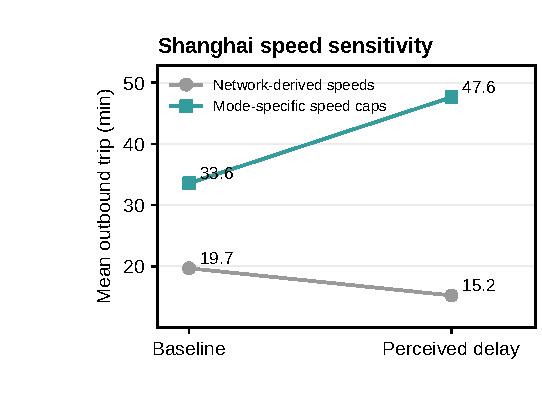
\includegraphics[width=.57\textwidth]{figures/narrative/figureS_speed_sensitivity.pdf}
\caption{Sensitivity of Shanghai journey times to the speeds of walking and cycling in the simulation. People, assigned modes, departure times and physical timetables are identical across speed settings. Values are mean durations of completed outbound trips.}
\label{fig:speed_sensitivity}
\end{figure}

\subsection{Singapore population responses and journey measures}
The Singapore scenario experiment simulates 10,000 synthetic travelers on unchanged physical supply. Scenario C0 is the baseline, C1 introduces heavy rain, C2 a 50\% fare increase and C3 a perceived PT delay of 15 minutes. C4 represents a road disruption that adds 20 minutes of car travel time and 20 minutes of reliability delay, and C5 combines rain with PT delay. Populations drawn with seeds 2026, 42 and 7 vary the composition of travelers, and MATSim uses seed 4711. Table~\ref{tab:singapore} gives the exact shares shown in Figure~\ref{main-fig:concept} of the main article, and Table~\ref{tab:seeds} their sensitivity to population composition.
\begin{table}[pos=htbp]
\centering\small
\setlength{\tabcolsep}{3pt}
\caption{Singapore absolute Student decision shares (percent) and MATSim consequences. Time is the completed-leg mean, not the mean journey duration per person. Seed 2026, 10,000 agents.}
\label{tab:singapore}
\begin{tabular}{@{}lrrrrrrr@{}}
\toprule
Scenario & Car & PT & Bike & Walk & Boardings & Car VKT (km) & \shortstack{Completed-leg\\mean (min)} \\
\midrule
C0 & 28.3 & 25.3 & 34.0 & 12.4 & 5613 & 33,939.0 & 43.67 \\
C1 & 37.6 & 45.3 & 13.3 & 3.8 & 9761 & 42,777.5 & 50.86 \\
C2 & 29.9 & 25.7 & 32.6 & 11.8 & 5674 & 35,797.8 & 43.86 \\
C3 & 29.0 & 10.3 & 35.8 & 25.0 & 2474 & 34,684.6 & 32.23 \\
C4 & 1.8 & 37.5 & 41.8 & 19.0 & 8537 & 2,943.4 & 52.71 \\
C5 & 37.7 & 18.6 & 24.5 & 19.2 & 4301 & 42,822.8 & 38.27 \\
\bottomrule
\end{tabular}
\end{table}

\begin{table}[pos=htbp]
\centering\small
\caption{Paired population-seed responses from the existing multi-seed summary.}
\label{tab:seeds}
\begin{tabular}{@{}lrrr@{}}
\toprule
Scenario & Seed & $\Delta$ PT pp & $\Delta$ car pp \\
\midrule
C1 & 2026 & +20.0 & +9.3 \\
C1 & 42 & +19.7 & +9.2 \\
C1 & 7 & +20.1 & +9.2 \\
C2 & 2026 & +0.4 & +1.6 \\
C2 & 42 & +0.5 & +1.8 \\
C2 & 7 & +0.5 & +1.5 \\
C3 & 2026 & -15.1 & +0.8 \\
C3 & 42 & -15.3 & +0.6 \\
C3 & 7 & -15.7 & +0.6 \\
C4 & 2026 & +12.1 & -26.5 \\
C4 & 42 & +11.7 & -26.1 \\
C4 & 7 & +12.3 & -26.5 \\
C5 & 2026 & -6.7 & +9.4 \\
C5 & 42 & -6.4 & +9.3 \\
C5 & 7 & -6.9 & +9.1 \\
\bottomrule
\end{tabular}
\end{table}

Journey measures for each person run from the first departure to the first activity other than home or an interaction point created by routing, such as a transfer. Table~\ref{tab:singapore_person_counts} reports people, boardings and legs separately. At baseline, 9,741 people complete the outbound journey and 9,062 return home. A completed outbound journey takes 66.43 minutes on average, whereas a completed leg takes 43.67 minutes, because a PT journey can consist of several legs.

Table~\ref{tab:singapore_person_time} also reports, for every departing person, the time elapsed until completion or until the end of the 30-hour simulation, a descriptive measure that includes unfinished journeys. Paired differences between scenarios use people who complete both trips and 4,000 paired-person resamples. All times reflect the network-based speeds and the fixed supply.
\begin{table}[pos=htbp]
\centering\footnotesize
\caption{Person and leg counts across six Singapore scenarios.}
\label{tab:singapore_person_counts}
\setlength{\tabcolsep}{3pt}
\renewcommand{\arraystretch}{1.15}
\begin{tabular}{@{}lrrrrrrr@{}}
\toprule
Scenario & \shortstack{Outbound\\complete} & \shortstack{Return\\complete} & \shortstack{Outbound\\PT people} & Boardings & \shortstack{Unfinished\\legs} & \shortstack{Stuck\\people} & \shortstack{Completed\\legs} \\
\midrule
C0 & 9,741 & 9,062 & 2,456 & 5,613 & 938 & 211 & 29,476 \\
C1 & 9,546 & 8,367 & 4,442 & 9,761 & 1,633 & 366 & 36,477 \\
C2 & 9,730 & 9,044 & 2,492 & 5,674 & 956 & 221 & 29,567 \\
C3 & 9,884 & 9,600 & 961 & 2,474 & 400 & 102 & 24,219 \\
C4 & 9,647 & 8,619 & 3,671 & 8,537 & 1,381 & 285 & 34,499 \\
C5 & 9,789 & 9,268 & 1,779 & 4,301 & 732 & 183 & 27,266 \\
\bottomrule
\end{tabular}
\par\smallskip\begin{minipage}{0.98\textwidth}\footnotesize Each scenario starts with and departs all 10,000 people. Completion and PT use are person counts. Boardings include transfers and both travel directions; unfinished legs and completed legs are different event-level counts. A stuck person may also have an unfinished leg.\end{minipage}
\end{table}

\begin{table}[pos=htbp]
\centering\footnotesize
\caption{Singapore timing with explicit units and completion conditions. All times are in minutes.}
\label{tab:singapore_person_time}
\setlength{\tabcolsep}{3pt}
\renewcommand{\arraystretch}{1.15}
\begin{tabular}{@{}lrrrrrl@{}}
\toprule
Scenario & \shortstack{Completed-leg\\mean} & \shortstack{Outbound\\mean} & \shortstack{Outbound\\median} & \shortstack{Completion-or-\\horizon mean} & \shortstack{Paired\\people} & \shortstack{Paired outbound change\\versus C0 [95\% CI]} \\
\midrule
C0 & 43.67 & 66.43 & 17.45 & 88.80 & -- & -- \\
C1 & 50.86 & 98.50 & 20.19 & 135.60 & 9,511 & +32.00 [+29.17, +34.69] \\
C2 & 43.86 & 66.88 & 16.97 & 90.01 & 9,708 & +0.60 [-0.45, +1.69] \\
C3 & 32.23 & 38.92 & 15.67 & 49.78 & 9,724 & -27.68 [-29.86, -25.56] \\
C4 & 52.71 & 94.78 & 27.08 & 124.21 & 9,578 & +28.39 [+25.98, +30.83] \\
C5 & 38.27 & 53.33 & 14.35 & 71.97 & 9,695 & -13.87 [-15.83, -11.96] \\
\bottomrule
\end{tabular}
\par\smallskip\begin{minipage}{0.98\textwidth}\footnotesize Outbound means and medians condition on the scenario-specific completers in Table~\ref{tab:singapore_person_counts}; the horizon mean retains all 10,000 departed people until completion or the administrative end at simulation hour 30. Paired changes retain only people completing both outbound journeys and use 4,000 paired-person bootstrap resamples (seed 917). The link-speed implementation limits interpretation as calibrated travel time.\end{minipage}
\end{table}

\FloatBarrier

\subsection{Feasibility correction and response geometry}
\label{sec:feasibility_geometry}
For a normalized distribution $\mathbf p$ and feasible set $F$ with mass $Z>0$, conditional renormalization adds mass $1-Z$ within $F$ and removes mass $1-Z$ outside it. Hence $\|\mathbf q-\mathbf p\|_1=2(1-Z)$. Every distribution supported on $F$ must remove all outside mass, and its inside changes have a sum of $1-Z$; the triangle inequality therefore gives the same lower bound. Conditional renormalization attains it, though the $L_1$ minimizer need not be unique.

An endpoint-optimal correction need not preserve a paired response. For a fixed feasible set $F=\{1,2\}$, let baseline probabilities be $(0.4,0.3,0.3)$ and perturbed probabilities $(0.4,0.2,0.4)$. Their corrections are $(4/7,3/7,0)$ and $(2/3,1/3,0)$. The probability of mode 1 is unchanged before correction but increases by $2/21$ afterward. This constructed example proves the distinction without making a claim about its empirical prevalence. The main-text decomposition reports the specified correction separately from subsequent execution; it does not attribute every correction-induced response difference to an unavoidable lower bound.
\FloatBarrier

\section{Computational measurements}
\label{sec:supp_compute}
Inference time for choice and timing together is measured on the 437 test states after feature encoding, using two CPU threads. After five untimed calls, 30 batches are timed, and the median batch time is divided by 437 for each seed (Table~\ref{tab:departure_runs}). MNL-S with neural timing requires $1.68\pm0.33$ microseconds per state, compared with $0.19\pm0.002$ with bounded-linear timing and 1.78--2.16 microseconds for the joint neural Students. Feature encoding and route preparation are not included.

The Teacher and SA-Student are compared on the same first 100 states, queried one at a time. The Teacher answers 87 of the 100 requests successfully, taking 86.539 seconds per successful request on average (95\% bootstrap interval 76.745--96.550), whereas SA-Student takes 0.272 milliseconds per state on a local processor. Neither figure includes the construction of a full population. Table~\ref{tab:inference_timing} distinguishes measured values from values scaled to larger populations.
\begin{table}[pos=htbp]
\centering\small
\caption{Time required for behavioral prediction alone. Teacher latency refers to successful requests, and Student times exclude supply preparation. Values for 10,000 agents are scaled or projected, not measured constructions.}
\label{tab:inference_timing}
\begin{tabularx}{\textwidth}{@{}lXrr@{}}
\toprule
Model & Measurement & Mean latency & 10,000 equivalent \\
\midrule
Teacher (remote) & 100 attempts, 87 successes & 86.539 s & 240.4 h (projected) \\
SA-Student sequential & Same first 100 states, one CPU thread & 0.272 ms & -- \\
SA-Student sequential & 100,000 states, one CPU thread & 0.332 ms & 3.3 s (scaled) \\
SA-Student batch 256 & 20,000 states, 24 CPU threads & 25,399 states/s & 0.4 s (scaled) \\
\bottomrule
\end{tabularx}
\end{table}

The nested Singapore populations contain 1,000, 10,000, 20,000 and 50,000 people, simulated with flow and storage capacity factors of 0.3 throughout (Table~\ref{tab:scale_full}). Construction time covers feature preparation, behavioral prediction and plan generation. The value for 1,000 people is the median of three constructions with identical behavioral predictions. Because larger populations also load the network more heavily at unchanged capacity factors, their simulation times do not correspond to calibrated city populations.
\begin{table}[pos=htbp]
\centering\small
\setlength{\tabcolsep}{3pt}
\caption{Population-scale construction and transport outcomes under unchanged Singapore supply, C0, seed 2026. Leg time averages completed legs, and unfinished legs count departures without a matching arrival. Smaller populations are subsets of larger ones, and the 1,000-agent row is the median of three constructions.}
\label{tab:scale_full}
\begin{tabular}{@{}rrrrrrr@{}}
\toprule
Agents & Build (min) & Decisions (s) & MATSim (min) & Boardings & \shortstack{Unfinished\\legs} & \shortstack{Completed-leg\\mean (min)} \\
\midrule
1,000 & 5.9 & 1.0 & 2.4 & 560 & 98 & 43.82 \\
10,000 & 51.1 & 10.3 & 2.1 & 5,613 & 938 & 43.67 \\
20,000 & 98.9 & 18.8 & 2.4 & 11,357 & 1,956 & 43.90 \\
50,000 & 231.8 & 48.8 & 3.4 & 28,440 & 5,586 & 48.92 \\
\bottomrule
\end{tabular}
\end{table}


Construction with and without reuse is compared for the same population and scenario. With reuse, route and accessibility calculations that depend only on the network and timetable are taken from an earlier construction, while Student predictions are recomputed. Construction time falls from 3,223.6 to 469.5 seconds in Singapore and from 10,491.8 to 103.2 seconds in Helsinki (Table~\ref{tab:pipeline}). All 10,000 mode and origin--destination assignments are unchanged, and only two Singapore departures and one Helsinki departure differ, by 0.01 minutes after rounding.
\begin{table}[pos=htbp]
\centering\small
\caption{Scenario-construction time for 10,000 agents without (cold) and with (warm) reuse of unchanged network and timetable calculations. Student predictions are recomputed in both cases.}
\label{tab:pipeline}
\begin{tabular}{@{}lrrrr@{}}
\toprule
City & Original (s) & Cold (s) & Warm (s) & Cold/warm \\
\midrule
Singapore & 3,063.1 & 3,223.6 & 469.5 & 6.9 \\
Helsinki & 9,507.0 & 10,491.8 & 103.2 & 101.7 \\
\bottomrule
\end{tabular}
\end{table}

All constructions ran on a machine with 24 logical CPU cores and 31.4 GB of memory, using PyTorch without GPU acceleration. Each city was measured once with reuse. The 50,000-person construction partly overlapped a preliminary Helsinki run, and one Helsinki delay construction shared the machine with other work, so these timings describe this machine under its recorded workload. The full cost of distillation would also include acquisition and retry charges that were not recorded in full. The retrospective accounting below uses available usage records and does not fill missing charges with zeros. The largest simulated population has 50,000 people, and the separate measurement on 100,000 states concerns inference alone.
\FloatBarrier

\subsection{Retrospective token accounting}
The accounting script reads retained repeat and API-call records, deduplicates them by completion ID and exports only aggregate counts and file hashes. At peak rates, a completion with $T_h$ cached input tokens, $T_m$ uncached input tokens and $T_o$ output tokens is repriced as
\begin{equation}
 C_{\mathrm{API}}=(0.044T_h+1.32T_m+3.96T_o)/10^6\quad\mathrm{USD}.
\end{equation}
Off-peak rates are half these values. These are the provider's rates checked on 25 September 2026, not a currency conversion or recovered invoice. The separately published CNY rates give CNY 700.30--1,400.61 for the same retained metered total. Promotions, account credits, tax treatment and unmetered requests are not reconstructed. The reproducible aggregate ledger is included with the manuscript under \path{reproduction/cost_audit/}; it contains no participant-level payloads.

The final same-task campaign made 2,880 recorded attempts: 1,440 valid responses and 1,440 HTTP 402 failures without usage. Its metered responses contain 1,409,152 cached and 915,218 uncached input tokens and 3,254,670 output tokens. Unknown charges for failures are not asserted to be zero. The earlier generic-prompt campaign had 1,475 usage-bearing responses, of which 35 were rejected by parsing; their tokens remain in the cost sum. The final campaign consumed an average of 1,614 input and 2,260 output tokens per valid response, which can inform a workload-matched budget but is not a guaranteed token ceiling for other prompts.

The 12 retained controlled-neural training status files report 29.58--32.13 seconds per fit on the recorded CPU setup, or 371.09 seconds summed over the fits. This sum is historical fit time, not elapsed campaign time or the complete training and adaptation history. No hardware rental or electricity charge was recorded. For reuse, the original acquisition cost is sunk; retraining from frozen targets adds no Teacher calls, while collecting new targets must be budgeted separately.

\section{Model roles, input sources and research materials}
\label{sec:materials_scope}

\subsection{Model roles and input sources}
Table~\ref{tab:model_roles} summarizes how the three model families enter the study, and Table~\ref{tab:input_provenance} the sources of information in the stated-choice inputs. Fitting settings and the numerical task specifications are given in Sections~\ref{sec:supp_controlled}, \ref{sec:s9_recipe} and~\ref{sec:supp_inputs}.

\begin{table}[pos=htbp]
\centering\small
\caption{Model families, their estimation and their role in the study.}
\label{tab:model_roles}
\renewcommand{\arraystretch}{1.13}
\begin{tabularx}{\linewidth}{@{}>{\raggedright\arraybackslash}p{0.19\linewidth}>{\raggedright\arraybackslash}p{0.27\linewidth}>{\raggedright\arraybackslash}X@{}}
\toprule
Model family & Behavioral specification & Estimation and role \\
\midrule
Joint neural Students & Shared representations with separate choice and departure outputs & Four objectives trained under matched conditions isolate the effect of the loss. Probability responses and timing are evaluated with separately selected fits. \\
MNL-S with separate timing & Linear choice utilities and an independently estimated timing predictor & Same inputs and training states, with a separately regularized choice model. Compares functional specifications and the separation of outcomes. \\
Supply-adapted Student & Adapted joint neural model with additional PT attributes & Differs in initialization, objective, auxiliary supervision and treatment of availability. Evaluated as an additional model, not as part of the matched loss comparison. \\
\bottomrule
\end{tabularx}
\end{table}

\begin{table}[pos=htbp]
\centering\small
\caption{Sources of information in the stated-choice model inputs.}
\label{tab:input_provenance}
\renewcommand{\arraystretch}{1.13}
\begin{tabularx}{\linewidth}{@{}>{\raggedright\arraybackslash}p{0.22\linewidth}>{\raggedright\arraybackslash}p{0.43\linewidth}>{\raggedright\arraybackslash}X@{}}
\toprule
Source & Information used & Interpretation \\
\midrule
Shown in the questionnaire & Singapore time and cost tables; the Shanghai PT fare of 6 yuan, parking fee of 30 yuan and one transfer & Attributes presented to respondents, with different numerical detail in the two surveys. \\
Reported by respondents & Personal characteristics supplied by respondents and covered by the model's input mapping & Observed inputs, although not every model attribute was collected. \\
Specified by the researchers & Characteristics not collected, and Shanghai durations and time components not shown in the tasks & Analysis assumptions. The twelve Singapore and eight Shanghai profiles examine selected alternatives rather than a full uncertainty distribution. \\
\bottomrule
\end{tabularx}
\end{table}
\FloatBarrier

\subsection{Versioned materials and reproduction tasks}
The material inventory refers to the repository edition of 24 September 2026 at commit
\begin{center}\small\texttt{4e67286ce72680a9e3a916a3fb7e97b1548b53f7}.\end{center}
The repository is \url{https://github.com/AnXu-ITS/DeepSeek_Traveler_Behavior_Distillation_Research}. It remains access-controlled. Its \path{docs/REPRODUCIBILITY.md} maps materials to reproduction tasks, and \path{evidence/paper_20260924/} contains the artifact manifest, verification record and compact numerical evidence. The manuscript source package separately contains input definitions, adaptation settings, editable figures and tabulated summaries.

\begin{table}[pos=htbp]
\centering\small
\caption{Teacher targets, reference-model provenance and supporting materials. Frozen-target re-evaluation and live-API replication are distinct tasks.}
\label{tab:teacher_materials}
\renewcommand{\arraystretch}{1.13}
\begin{tabularx}{\linewidth}{@{}>{\raggedright\arraybackslash}p{0.18\linewidth}>{\raggedright\arraybackslash}p{0.30\linewidth}>{\raggedright\arraybackslash}X@{}}
\toprule
Use & Coverage & Materials and interpretation \\
\midrule
Controlled supervision & 437 test states; repeat analysis covers 373 states and 350 pairs. & Prepared states, aggregate targets, splits, 12 selected neural fits, MNL-S records and evaluation code are included. Individual repeats are unavailable for the 64 mechanism states; the authors identify the service as official DeepSeek V4 Pro, while immutable per-response backend identity is not retained for every target. \\
Supply adaptation & 336 accessibility states; 1,502 valid queries. & Adaptation specification and released SA-Student and predecessor checkpoints are included. Retained response records and training history support the adaptation provenance. \\
Contemporary API reference & 24 respondents per city; ten tasks; three successful elicitations per state. & Configuration, prompt, campaign summary and aggregate comparisons are included. The returned model string is the alias \texttt{deepseek-v4-pro}; participant-linked payloads are retained separately. The alias alone does not establish backend identity. \\
\bottomrule
\end{tabularx}
\end{table}

The authors confirm use of the official DeepSeek V4 Pro service throughout collection. The API documentation, checked on 25 September 2026, explicitly retains Pro service after 14 September and identifies the model as DeepSeek-V4-Pro-0813. This supersedes the routing assumption in the earlier editorial draft. The historical news page and the revised API documentation are not consistent on the announced routing plan; we use the updated service documentation and retained request records for attribution rather than infer that these experiments used Flash. The deduplicated supervision archives retain completion creation times from 21 August to 27 August 2026 (UTC), while the final same-task reference completions were created on 21 September 2026 from 16:35:54 to 17:01:40 UTC. These are provider creation times, not selection seeds. The final campaign has 1,440 usage-bearing responses, all returning \texttt{deepseek-v4-pro}, and each recorded request specifies 16,384 maximum tokens. Its copied campaign configuration reports 8,192; the request-level fields take precedence for this batch. Early repeat records do not retain a response model field, and immutable backend fingerprints are incomplete. Frozen targets therefore remain the basis for exact target-based re-evaluation; service identity alone does not turn the later comparison into a causal estimate of compression error.

\paragraph{Controlled-model evaluation.}
The prepared benchmark is in \path{outputs/matched_response_v1/bundle/}, selected neural fits in \path{outputs/matched_response_v1/train/}, and modular fits in \path{outputs/revision_20260921/baselines/}. Local inference uses a synthetic example and a frozen checkpoint. The archived-checkpoint helper extracts the recorded source and checks its fingerprint before evaluation. Historical fingerprints depend on platform-specific path separators; portability changes should be versioned rather than treated as exact replay. The repository's retained verification record reports local inference and re-evaluation of two selected neural checkpoints, not a new full training campaign.

\paragraph{Survey analyses.}
The repository includes the English questionnaire instruments, complete aggregate contrast tables and analysis implementations. Reproducing respondent-level resampling or participant-linked Teacher comparisons requires the separately retained participant records and appropriate privacy-aware access. Aggregate-table inspection is distinct from re-estimation of participant-level intervals. These restrictions do not apply to the synthetic benchmark targets and released model weights.

\paragraph{Network execution.}
The repository includes the 140-run ledger, 70 paired summaries, experiment driver and event-analysis code. Fresh Helsinki execution requires the fixed population, prepared road/transit supply and Java/MATSim runtime; the full event archive, approximately 57.5 GB, is retained separately. The implementation is specified by \path{scripts/revision_20260921/helsinki_execution.py} and \path{src/traveler_distillation/matsim/adapter.py}. Dependency records are provided, although the historical stages do not share one fully locked environment.

The retained ledgers contain 1,000 people in each completed run and no zero-feasible-mass case. Across conditions, 2,006 outbound PT assignments and 940 car assignments fell back to walking; these are repeated traveler records, not distinct people. No recorded outbound or return walking route consisted only of its origin link. The general adapter can produce an origin-link-only walk after an unsuccessful walking search, so this tested behavior does not establish handling of disconnected networks. These ledger checks assess the completed runs; the repository expansion itself did not rerun all simulations.

Requests for access should be directed to the corresponding author, subject to participant privacy and third-party terms. The included manifest records artifact hashes and the material scope, while the verification record distinguishes executed checks from retained historical outputs. This inventory supersedes earlier availability text that predates the repository expansion.

\end{document}
